%%%%%%%%%%%%%%%%%%%%%%%%%%%%%%%%%%%%%%%%%
% Beamer Presentation
% LaTeX Template
% Version 1.0 (10/11/12)
%
% This template has been downloaded from:
% http://www.LaTeXTemplates.com
%
% License:
% CC BY-NC-SA 3.0 (http://creativecommons.org/licenses/by-nc-sa/3.0/)
%
%%%%%%%%%%%%%%%%%%%%%%%%%%%%%%%%%%%%%%%%%

%----------------------------------------------------------------------------------------
%	PACKAGES AND THEMES
%----------------------------------------------------------------------------------------

\documentclass[handout]{beamer}

\mode<presentation> {

% The Beamer class comes with a number of default slide themes
% which change the colors and layouts of slides. Below this is a list
% of all the themes, uncomment each in turn to see what they look like.

%\usetheme{default}
%\usetheme{AnnArbor}
%\usetheme{Antibes}
%\usetheme{Bergen}
%\usetheme{Berkeley}
%\usetheme{Berlin}
%\usetheme{Boadilla}
%\usetheme{CambridgeUS}
%\usetheme{Copenhagen}
%\usetheme{Darmstadt}
%\usetheme{Dresden}
%\usetheme{Frankfurt}
%\usetheme{Goettingen}
%\usetheme{Hannover}
%\usetheme{Ilmenau}
%\usetheme{JuanLesPins}
%\usetheme{Luebeck}
\usetheme{Madrid}
%\usetheme{Malmoe}
%\usetheme{Marburg}
%\usetheme{Montpellier}
%\usetheme{PaloAlto}
%\usetheme{Pittsburgh}
%\usetheme{Rochester}
%\usetheme{Singapore}
%\usetheme{Szeged}
%\usetheme{Warsaw}

% As well as themes, the Beamer class has a number of color themes
% for any slide theme. Uncomment each of these in turn to see how it
% changes the colors of your current slide theme.

%\usecolortheme{albatross}
%\usecolortheme{beaver}
%\usecolortheme{beetle}
%\usecolortheme{crane}
%\usecolortheme{dolphin}
%\usecolortheme{dove}
%\usecolortheme{fly}
%\usecolortheme{lily}
%\usecolortheme{orchid}
%\usecolortheme{rose}
%\usecolortheme{seagull}
%\usecolortheme{seahorse}
%\usecolortheme{whale}
%\usecolortheme{wolverine}

%\setbeamertemplate{footline} % To remove the footer line in all slides uncomment this line
%\setbeamertemplate{footline}[page number] % To replace the footer line in all slides with a simple slide count uncomment this line

%\setbeamertemplate{navigation symbols}{} % To remove the navigation symbols from the bottom of all slides uncomment this line
}

\usepackage{graphicx} % Allows including images
\usepackage{booktabs} % Allows the use of \toprule, \midrule and \bottomrule in tables
\usepackage{cool}
\usepackage{tikz}
\usepackage{amsmath}
\usepackage{pseudocode}
\usepackage{MnSymbol,wasysym}
\DeclareMathOperator*{\argmax}{argmax}
\DeclareMathOperator*{\argmin}{argmin}
\usetikzlibrary{positioning}

%----------------------------------------------------------------------------------------
%	TITLE PAGE
%----------------------------------------------------------------------------------------

\title[Optimal Order Execution]{Stochastic Control of Optimal Trade Order Execution} % The short title appears at the bottom of every slide, the full title is only on the title page

\author{Ashwin Rao} % Your name
\institute[Stanford] % Your institution as it will appear on the bottom of every slide, may be shorthand to save space
{
ICME, Stanford University
 % Your institution for the title page
}

\date{\today} % Date, can be changed to a custom date

\begin{document}
\begin{frame}
\titlepage % Print the title page as the first slide
\end{frame}

\begin{frame}
\frametitle{Overview} % Table of contents slide, comment this block out to remove it
\tableofcontents % Throughout your presentation, if you choose to use \section{} and \subsection{} commands, these will automatically be printed on this slide as an overview of your presentation
\end{frame}

\section{Order Book and Price Impact}

\begin{frame}
\frametitle{Trading Order Book}
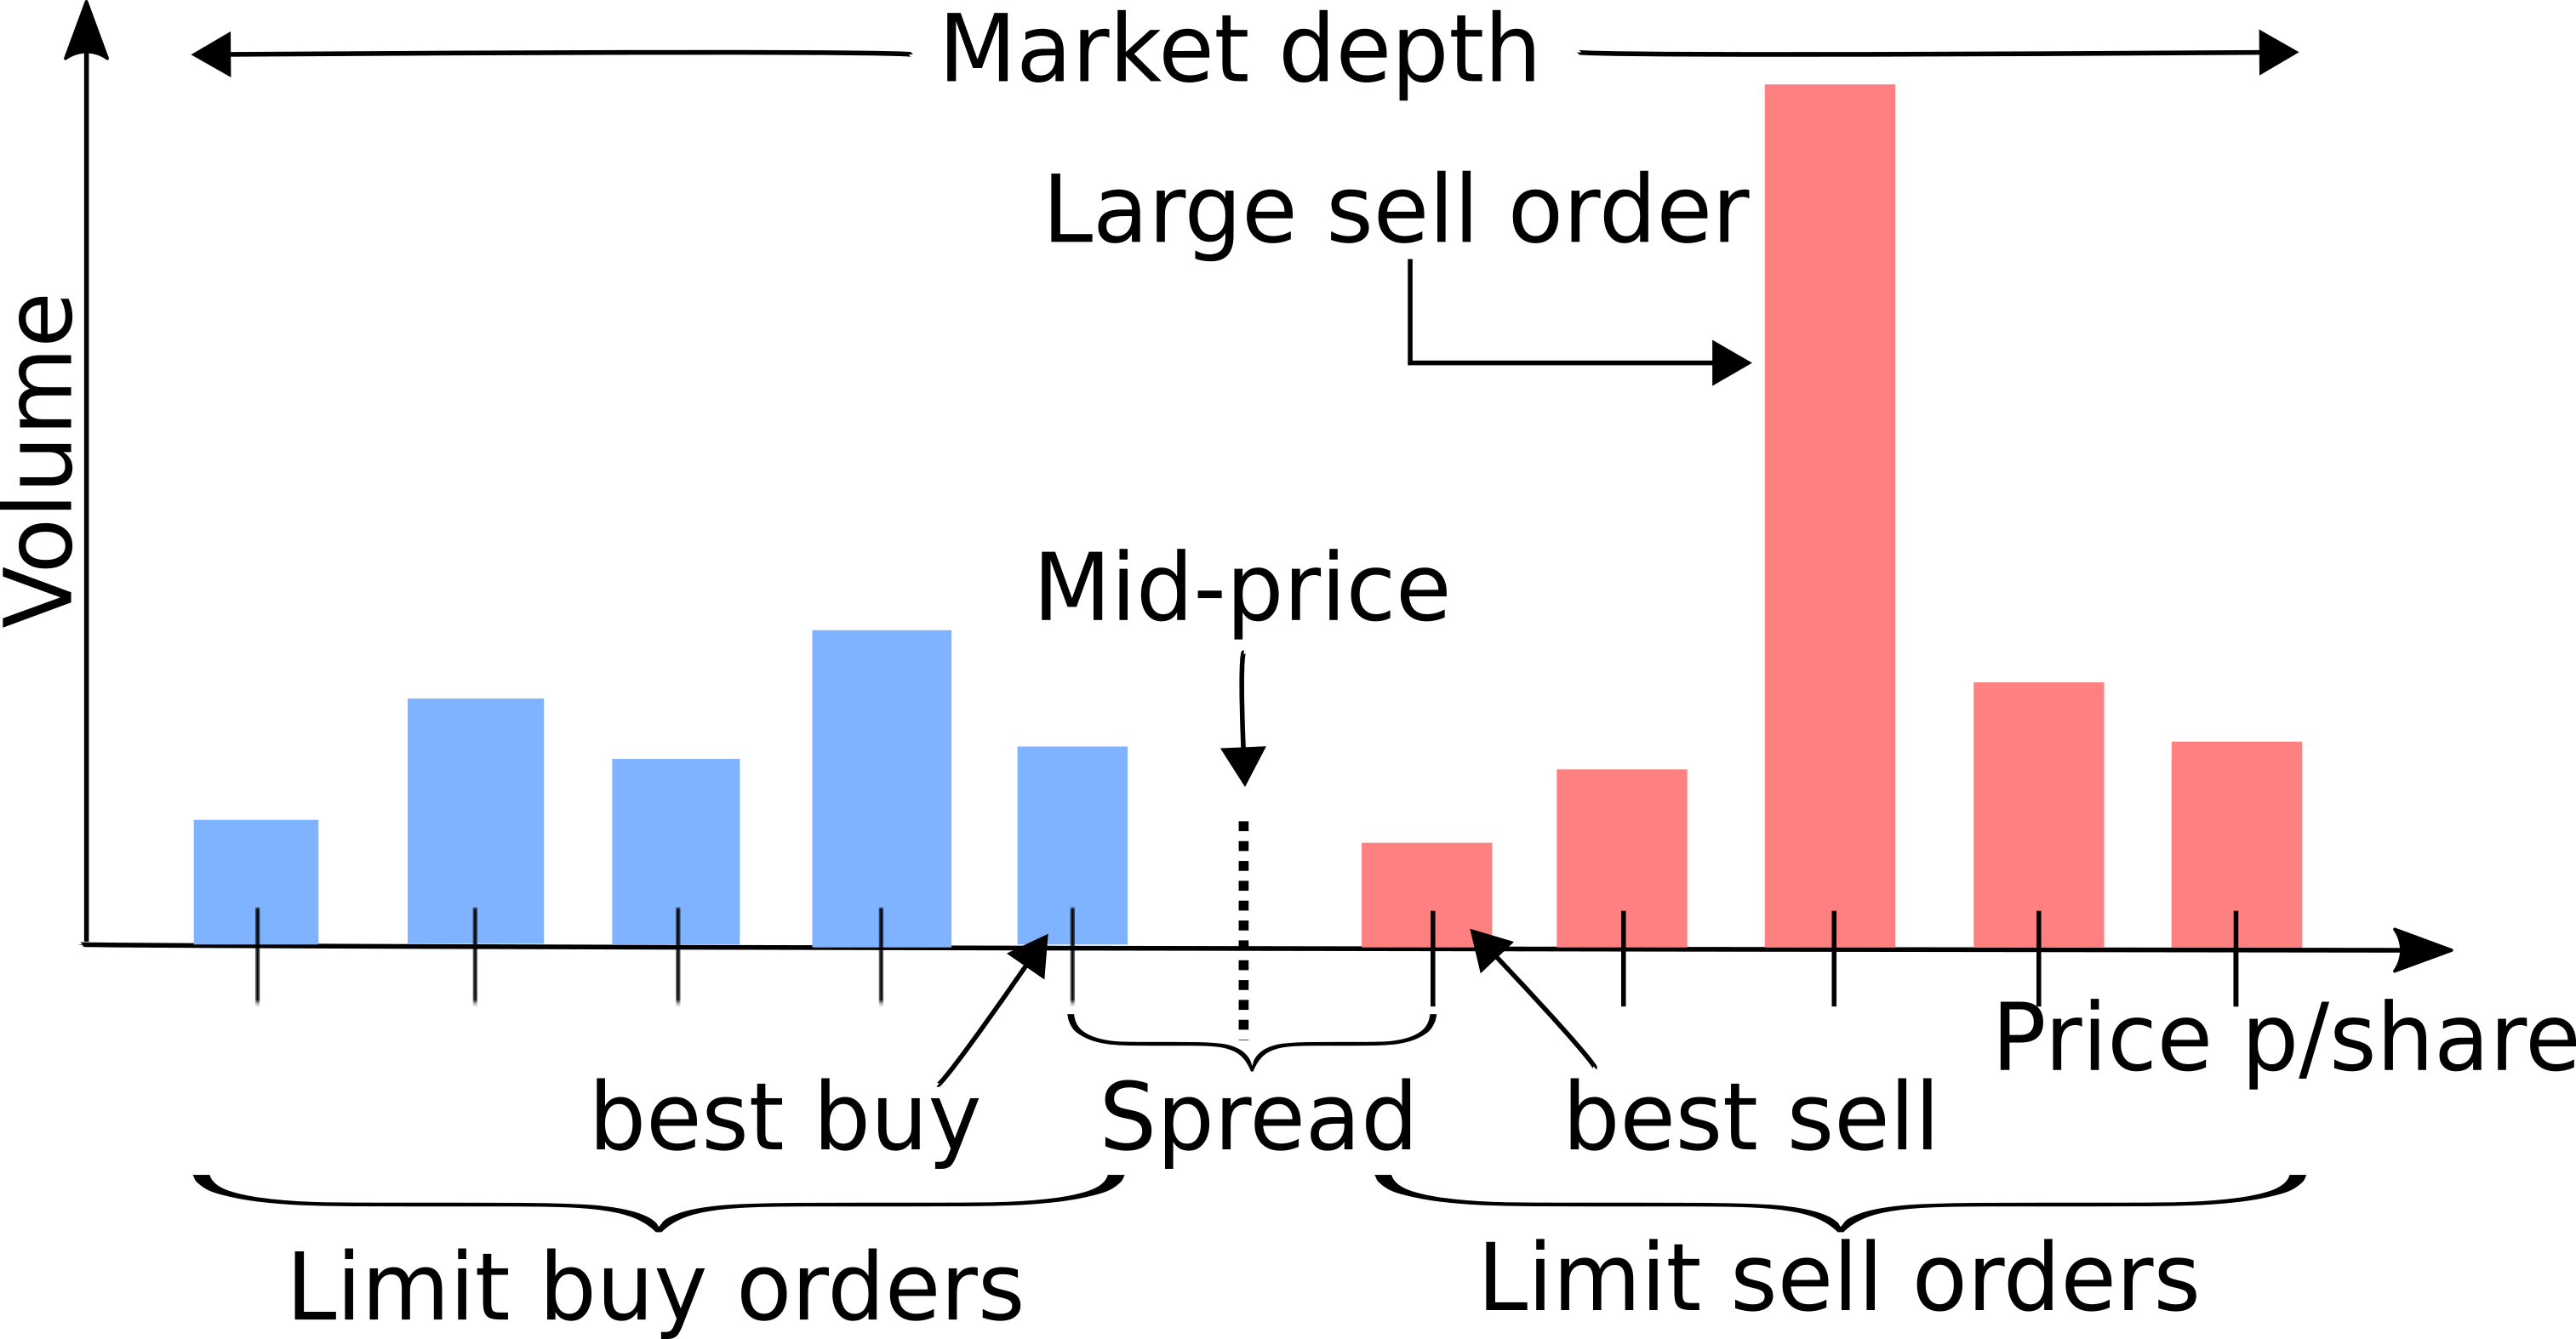
\includegraphics[width=11.5cm, height=7cm]{order_book.png}
\end{frame}

\begin{frame}
\frametitle{Basics of Trading Order Book}
\pause
\begin{itemize}[<+->]
\item Buyers/Sellers express their intent to trade by submitting bids/asks
\item These are Limit Orders (LO) with a price $P$ and size $N$
\item Buy LO $(P, N)$ states willingness to buy $N$ shares at a price $\leq P$
\item Sell  LO $(P, N)$ states willingness to sell $N$ shares at a price $\geq P$
\item Order Book (OB) aggregates order sizes for each unique price
\item So we can represent with two sorted lists of (Price, Size) pairs
$$\mbox{Bids: } [(P_i^{(b)}, N_i^{(b)}) \mid 1 \leq i \leq m], P_i^{(b)} > P_j^{(b)} \mbox{ for } i < j$$
$$\mbox{Asks: } [(P_i^{(a)}, N_i^{(a)}) \mid 1 \leq i \leq n], P_i^{(a)} < P_j^{(a)} \mbox{ for } i < j$$
\item We call $P_1^{(b)}$ as simply {\em Bid}, $P_1^{(a)}$ as {\em Ask}, $\frac {P_1^{(a)} + P_1^{(b)}} 2$ as {\em Mid}
\item We call $P_1^{(a)} - P_1^{(b)}$ as {\em Spread}, $P_n^{(a)} - P_m^{(b)}$ as {\em Market Depth}
\item A Market Order (MO) states intent to buy/sell $N$ shares at the {\em best possible price(s)} available on the OB at the time of MO submission
\end{itemize}
\end{frame}

\begin{frame}
\frametitle{Trading Order Book Activity}
\pause
\begin{itemize}[<+->]
\item A new Sell LO $(P,N)$ potentially removes best bid prices on the OB
$$\mbox{Removal: } [(P_i^{(b)}, \min(N_i^{(b)}, \max(0, N - \sum_{j=1}^{i-1} N_j^{(b)}))) \mid (i: P_i^{(b)} \geq P)]$$
\item After this removal, it will add the following to the asks side of the OB 
$$(P, \max(0, N - \sum_{i: P_i^{(b)} \geq P}  N_i^{(b)}))$$
\item A Sell Market Order $N$ will remove the best bid prices on the OB
$$\mbox{Removal: } [(P_i^{(b)}, \min(N_i^{(b)}, \max(0, N - \sum_{j=1}^{i-1} N_j^{(b)}))) \mid 1 \leq i \leq m]$$
\item A Buy Market Order $N$ will remove the best ask prices on the OB
$$\mbox{Removal: } [(P_i^{(a)}, \min(N_i^{(a)}, \max(0, N - \sum_{j=1}^{i-1} N_j^{(a)}))) \mid 1 \leq i \leq n]$$
\end{itemize}
\end{frame}

\begin{frame}
\frametitle{Price Impact and Order Book Dynamics}
\pause
\begin{itemize}[<+->]
\item We focus on how a Market order (MO) alters the order book
\item A large-sized MO often results in a big {\em Spread} which could soon be replenished by new LOs, potentially from either side
\item So a large-sized MO moves the Bid/Ask/Mid ({\em Price Impact} of MO)
\item Subsequent Replenishment activity is part of {\em Order Book Dynamics}
\item Models for Order Book Dynamics can be quite complex
\item We will cover a few simple Models in this lecture
\item Models based on how a Sell MO will move the OB {\em Bid Price}
\item Models of Buy MO moving the OB {\em Ask Price} are analogous
\end{itemize}
\end{frame}

\section{Definition of Optimal Trade Order Execution Problem}

\begin{frame}
\frametitle{Optimal Trade Order Execution Problem}
\pause
\begin{itemize}[<+->]
\item The task is to sell a large number $N$ of shares
\item We are allowed to trade in $T$ discrete time steps
\item We are only allowed to submit Market Orders
\item We consider both {\em Temporary} and {\em Permanent} Price Impact
\item For simplicity, we consider a model of just the {\em Bid Price} Dynamics
\item Goal is to maximize Expected Total Utility of Sales Proceeds
\item By breaking $N$ into appropriate chunks (timed appropriately)
\item If we sell too fast, we are likely to get poor prices
\item If we sell too slow, we risk running out of time
\item Selling slowly also leads to more uncertain proceeds (lower Utility)
\item This is a Dynamic Optimization problem
\item We can model this problem as a Markov Decision Process (MDP)
\end{itemize}
\end{frame}

\begin{frame}
\frametitle{Problem Notation}
\pause
\begin{itemize}[<+->]
\item Time steps indexed by $t = 1, \ldots, T$
\item $P_t$ denotes Bid Price at start of time step $t$
\item $N_t$ denotes number of shares sold in time step $t$
\item $R_t = N - \sum_{i=1}^{t-1}N_i = $ shares remaining to be sold at start of time step $t$
\item Note that $R_1 = N, N_T = R_T$
\item Price Dynamics given by:
$$P_{t+1} = f_t(P_t, N_t, \epsilon_t)$$
where $f_t(\cdot)$ is an arbitrary function incorporating:
\begin{itemize}
\item Permanent Price Impact of selling $N_t$ shares
\item Impact-independent market-movement of Bid Price over time step $t$
\item $\epsilon_t$ denotes source of randomness in Bid Price market-movement
\end{itemize}
\item Sales Proceeds in time step $t$ defined as:
$$N_t \cdot Q_t = N_t \cdot (P_t - g_t(P_t, N_t))$$
where $g_t(\cdot)$ is an arbitrary func representing Temporary Price Impact
\item Utility of Sales Proceeds function denoted as $U(\cdot)$
\end{itemize}
\end{frame}

\begin{frame}
\frametitle{Markov Decision Process (MDP) Formulation}
\pause
\begin{itemize}[<+->]
\item Order of MDP activity in each time step $1 \leq t \leq T$:
\begin{itemize}
\item Observe {\em State} $:= (t, P_t, R_t)$
\item Perform {\em Action} $:= N_t$
\item Receive {\em Reward} $:= U(N_t \cdot Q_t) = U(N_t \cdot (P_t - g_t(P_t, N_t)))$
\item Experience Price Dynamics $P_{t+1} = f_t(P_t, N_t, \epsilon_t)$
\end{itemize}
\item Goal is to find a Policy $\pi^*(t, P_t, R_t) = N_t$ that maximizes: $$\mathbb{E}[\sum_{t=1}^T \gamma^t \cdot U(N_t \cdot Q_t)] \mbox{ where } \gamma \mbox{ is MDP discount factor}$$
\end{itemize}
\end{frame}

\section{Simple Models, leading to Analytical Solutions}

\begin{frame}
\frametitle{A Simple Linear Impact Model with No Risk-Aversion}
\pause
\begin{itemize}[<+->]
\item We consider a simple model with Linear Price Impact
\item $N, N_t, P_t$ are all continuous-valued ($\in \mathbb{R}$)
\item In particular, we allow $N_t$ to be possibly negative (unconstrained)
\item Price Dynamics: $P_{t+1} = P_t - \alpha N_t + \epsilon_t$ where $\alpha \in \mathbb{R}^+$
\item $\epsilon_t$ is i.i.d. with $\mathbb{E}[\epsilon_t|N_t, P_t] = 0$
\item So, Permanent Price Impact is $\alpha N_t$
\item Temporary Price Impact given by $\beta N_t$, so $Q_t = P_t - \beta N_t$ ($\beta \in \mathbb{R}^+$)
\item Utility function $U(\cdot)$ is the identity function, i.e., no Risk-Aversion
\item MDP Discount factor $\gamma = 1$
\item This is an unrealistic model, but solving this gives plenty of intuition
\item Approach: Define Optimal Value Function \& invoke Bellman Equation
\end{itemize}
\end{frame}

\begin{frame}
\frametitle{Optimal Value Function and Bellman Equation}
\pause
\begin{itemize}
\item Denote Value Function for policy $\pi$ as: $$V^{\pi}(t, P_t, R_t) = \mathbb{E}_{\pi}[\sum_{i=t}^T N_i (P_i - \beta N_i)|(t,P_t,R_t)]$$
\pause
\item Denote Optimal Value Function as $V^*(t,P_t,R_t) = max_{\pi} V^{\pi}(t,P_t,R_t)$
\pause
\item Optimal Value Function satisfies the Bellman Equation ($\forall 1 \leq t < T$):
$$V^*(t,P_t,R_t) = \max_{N_t} (N_t(P_t - \beta N_t)  + \mathbb{E}[V^*(t+1, P_{t+1}, R_{t+1})])$$
\pause
$$\mbox{Note: } V^*(T, P_T,R_T) = R_T(P_T - \beta R_T)$$
\item From the above, we can infer $V^*(T-1,P_{T-1},R_{T-1})$ as:
$$\max_{N_{T-1}} \{ N_{T-1}(P_{T-1} - \beta N_{T-1})  + \mathbb{E}[R_T(P_T - \beta R_T)] \}$$
\end{itemize}
$$=\max_{N_{T-1}} \{ N_{T-1}(P_{T-1} - \beta N_{T-1})  + \mathbb{E}[(R_{T-1} - N_{T-1})(P_T - \beta(R_{T-1} - N_{T-1})) \}$$
$$=\max_{N_{T-1}} \{ N_{T-1}(P_{T-1} - \beta N_{T-1})  + (R_{T-1} - N_{T-1})(P_{T-1} - \alpha N_{T-1} - \beta(R_{T-1} - N_{T-1})) \}$$
\end{frame}

\begin{frame}
\frametitle{Optimal Policy and Optimal Value Function}
\pause
\begin{itemize}
\item Differentiating this expression w.r.t. $N_{T-1}$ and setting to 0 gives:
$$2N^*_{T-1} (\alpha - 2\beta) - R_{T-1}(\alpha - 2\beta) = 0 \Rightarrow N^*_{T-1} = \frac {R_{T-1}} 2$$
\pause
\item Substitute $N^*_{T-1}$ in the expression for $V^*(T-1,P_{T-1},R_{T-1})$:
$$V^*(T-1,P_{T-1},R_{T-1}) =  R_{T-1} P_{T-1} - R_{T-1}^2 (\frac {\alpha + 2\beta} 4)$$
\pause
\item Continuing backwards in time in this manner gives:
$$N^*_t = \frac {R_t} {T-t+1}$$
\pause
$$V^*(t, P_t,R_t) = R_t P_t - \frac {R_t^2} 2 (\frac {2\beta + (T-t)\alpha} {T-t+1})$$
\end{itemize}
\end{frame}

\begin{frame}
\frametitle{Interpreting the solution}
\pause
\begin{itemize}[<+->]
\item Rolling forward in time, we see that $N^*_t = \frac N T$, i.e., uniformly split
\item Hence, Optimal Policy is a constant (independent of {\em State})
\item Uniform split makes intuitive sense because Price Impact and Market Movement are both linear and additive, and don't interact
\item Essentially equivalent to minimizing $\sum_{t=1}^T N_t^2$ with $\sum_{t=1}^T N_t = N$
\item Optimal Expected Total Sale Proceeds $= NP_1 - \frac {N^2} 2 (\alpha + \frac {2\beta - \alpha} T)$
\item So, {\em Implementation Shortfall} from Price Impact is $\frac {N^2} 2 (\alpha + \frac {2\beta - \alpha} T)$
\item Note that Implementation Shortfall is non-zero ($\frac {\alpha N^2} 2$) when $T\rightarrow \infty$
\item This is because we assumed non-zero {\em Permanent Price Impact} ($\alpha \neq 0$)
\item If Price Impact were purely temporary (i.e., Price fully snapped back), Implementation Shortfall would be zero when $T\rightarrow \infty$
\end{itemize}
\end{frame}

\begin{frame}
\frametitle{Models in Bertsimas-Lo paper}
\pause
\begin{itemize}[<+->]
\item \href{http://alo.mit.edu/wp-content/uploads/2015/06/Optimal-Control-of-Execution-Costs.pdf}{\underline{\textcolor{blue}{Bertsimas-Lo}}} was the first paper on Optimal Trade Order Execution
\item They assumed no risk-aversion, i.e. identity Utility function
\item The first model in their paper is a special case of our simple Linear Impact model, with fully Permanent Impact (i.e., $\alpha = \beta$)
\item Next, Betsimas-Lo extended the Linear Permanent Impact model
\item To include dependence on Serially-Correlated Variable $X_t$
$$P_{t+1} = P_t - (\alpha N_t + \theta X_t) + \epsilon_t, X_{t+1} = \rho X_t + \eta_t, Q_t = P_t - (\alpha N_t + \theta X_t)$$
\item $\epsilon_t$ and $\eta_t$ are i.i.d. (and mutually independent) with mean zero
\item $X_t$ can be thought of as market factor affecting $P_t$ linearly
\item Bellman Equation on Optimal VF and same approach as before yields:
$$N^*_t = \frac {R_t} {T-t+1} + h(t, \alpha, \theta, \rho) X_t$$
$$V^*(t,P_t,R_t,X_t) = R_tP_t - (\mbox{quadratic in } (R_t,X_t) + \mbox{ constant})$$
\item Seral-correlation predictability ($\rho \neq 0$) alters uniform-split strategy
\end{itemize}
\end{frame}

\begin{frame}
\frametitle{A more Realistic Model: LPT Price Impact}
\pause
\begin{itemize}
\pause
\item Next, Bertsimas-Lo present a more realistic model called ``LPT''
\pause
\item {\em Linear-Percentage Temporary} Price Impact model features:
\pause
\begin{itemize}
\item Geometric random walk: consistent with real data, \& avoids prices $\leq 0$
\pause
\item \% Price Impact $\frac {g_t(P_t,N_t)} {P_t}$ doesn't depend on $P_t$ (validated by real data)
\pause
\item Purely Temporary Price Impact
\pause
\end{itemize}
$$P_{t+1} = P_t e^{Z_t},  X_{t+1} = \rho X_t + \eta_t, Q_t = P_t(1 - \alpha N_t - \theta X_t)$$
\pause
\item $Z_t$ is a random variable with mean $\mu_Z$ and variance $\sigma^2_Z$
\pause
\item With the same derivation as before, we get the solution:
$$N_t^* = c^{(1)}_t + c^{(2)}_t R_t + c^{(3)}_t X_t $$
\pause
\begin{align*}
V^*(t,P_t,R_t,X_t) = e^{\mu_Z + \frac {\sigma_Z^2} 2} \cdot P_t \cdot ( & c^{(4)}_t + c^{(5)}_t R_t + c^{(6)}_t X_t \\
& + c^{(7)}_t R_t^2 + c^{(8)}_t X_t^2 + c^{(9)}_t R_t X_t)\\
\end{align*}
\pause
\item $c^{(k)}_t, 1 \leq k \leq 9$ are independent of $P_t, R_t, X_t$
\end{itemize}
\end{frame}

\begin{frame}
\frametitle{Incorporating Risk-Aversion/Utility of Proceeds}
\pause
\begin{itemize}[<+->]
\item For analytical tractability, Bertsimas-Lo ignored Risk-Aversion
\item But one is typically wary of {\em Risk of Uncertain Proceeds}
\item We'd trade some (Expected) Proceeds for lower Variance of Proceeds
\item \href{https://www.math.nyu.edu/faculty/chriss/optliq_f.pdf}{\underline{\textcolor{blue}{Almgren-Chriss}}} work in this Risk-Aversion framework
\item They consider our simple linear model maximizing $E[Y] - \lambda Var[Y]$
\item Where $Y$ is the total (uncertain) proceeds $\sum_{i=1}^T N_i Q_i$
\item $\lambda$ controls the degree of risk-aversion and hence, the trajectory of $N_t^*$
\item $\lambda = 0$ leads to uniform split strategy $N_t^* = \frac N T$
\item The other extreme is to minimize $Var[Y]$ which yields $N_1^* = N$
\item Almgren-Chriss derive {\em Efficient Frontier} and solutions for specific $U(\cdot)$
\item Much like classical Portfolio Optimization problems
\end{itemize}
\end{frame}

\section{Real-World Considerations, Extensions, Reinforcement Learning}

\begin{frame}
\frametitle{Real-world Optimal Trade Order Execution (\& Extensions)}
\pause
\begin{itemize}[<+->]
\item Arbitrary Price Dynamics $f_t(\cdot)$ and Temporary Price Impact $g_t(\cdot)$
\item Non-stationarity/non-linear dynamics/impact require (Numerical) DP
\item Frictions: Discrete Prices/Sizes, Constraints on Prices/Sizes, Fees
\item Large State space to incorporate various external factors in the State
\item Need to utilize methods in Approximate Dynamic Programming
\item And if model is unknown/to be learnt, Reinforcement Learning
\item This problem can be extended in two important ways:
\begin{itemize}
\item State is {\em Complete Order Book} (Model of Order Book Dynamics)
\item Optimal Execution of a {\em Portfolio} (Cross-Asset Impact Modeling)
\end{itemize}
\item Can this be combined with Portfolio Optimization problem?
\item Can we exploit recent advances in Deep Reinforcement Learning?
\item Exciting area for Future Research as well as Engineering Design
\end{itemize}
\end{frame}

\end{document}
